% Options for packages loaded elsewhere
\PassOptionsToPackage{unicode}{hyperref}
\PassOptionsToPackage{hyphens}{url}
%
\documentclass[
]{article}
\usepackage{amsmath,amssymb}
\usepackage{lmodern}
\usepackage{ifxetex,ifluatex}
\ifnum 0\ifxetex 1\fi\ifluatex 1\fi=0 % if pdftex
  \usepackage[T1]{fontenc}
  \usepackage[utf8]{inputenc}
  \usepackage{textcomp} % provide euro and other symbols
\else % if luatex or xetex
  \usepackage{unicode-math}
  \defaultfontfeatures{Scale=MatchLowercase}
  \defaultfontfeatures[\rmfamily]{Ligatures=TeX,Scale=1}
\fi
% Use upquote if available, for straight quotes in verbatim environments
\IfFileExists{upquote.sty}{\usepackage{upquote}}{}
\IfFileExists{microtype.sty}{% use microtype if available
  \usepackage[]{microtype}
  \UseMicrotypeSet[protrusion]{basicmath} % disable protrusion for tt fonts
}{}
\makeatletter
\@ifundefined{KOMAClassName}{% if non-KOMA class
  \IfFileExists{parskip.sty}{%
    \usepackage{parskip}
  }{% else
    \setlength{\parindent}{0pt}
    \setlength{\parskip}{6pt plus 2pt minus 1pt}}
}{% if KOMA class
  \KOMAoptions{parskip=half}}
\makeatother
\usepackage{xcolor}
\IfFileExists{xurl.sty}{\usepackage{xurl}}{} % add URL line breaks if available
\IfFileExists{bookmark.sty}{\usepackage{bookmark}}{\usepackage{hyperref}}
\hypersetup{
  hidelinks,
  pdfcreator={LaTeX via pandoc}}
\urlstyle{same} % disable monospaced font for URLs
\usepackage[margin=1in]{geometry}
\usepackage{color}
\usepackage{fancyvrb}
\newcommand{\VerbBar}{|}
\newcommand{\VERB}{\Verb[commandchars=\\\{\}]}
\DefineVerbatimEnvironment{Highlighting}{Verbatim}{commandchars=\\\{\}}
% Add ',fontsize=\small' for more characters per line
\usepackage{framed}
\definecolor{shadecolor}{RGB}{248,248,248}
\newenvironment{Shaded}{\begin{snugshade}}{\end{snugshade}}
\newcommand{\AlertTok}[1]{\textcolor[rgb]{0.94,0.16,0.16}{#1}}
\newcommand{\AnnotationTok}[1]{\textcolor[rgb]{0.56,0.35,0.01}{\textbf{\textit{#1}}}}
\newcommand{\AttributeTok}[1]{\textcolor[rgb]{0.77,0.63,0.00}{#1}}
\newcommand{\BaseNTok}[1]{\textcolor[rgb]{0.00,0.00,0.81}{#1}}
\newcommand{\BuiltInTok}[1]{#1}
\newcommand{\CharTok}[1]{\textcolor[rgb]{0.31,0.60,0.02}{#1}}
\newcommand{\CommentTok}[1]{\textcolor[rgb]{0.56,0.35,0.01}{\textit{#1}}}
\newcommand{\CommentVarTok}[1]{\textcolor[rgb]{0.56,0.35,0.01}{\textbf{\textit{#1}}}}
\newcommand{\ConstantTok}[1]{\textcolor[rgb]{0.00,0.00,0.00}{#1}}
\newcommand{\ControlFlowTok}[1]{\textcolor[rgb]{0.13,0.29,0.53}{\textbf{#1}}}
\newcommand{\DataTypeTok}[1]{\textcolor[rgb]{0.13,0.29,0.53}{#1}}
\newcommand{\DecValTok}[1]{\textcolor[rgb]{0.00,0.00,0.81}{#1}}
\newcommand{\DocumentationTok}[1]{\textcolor[rgb]{0.56,0.35,0.01}{\textbf{\textit{#1}}}}
\newcommand{\ErrorTok}[1]{\textcolor[rgb]{0.64,0.00,0.00}{\textbf{#1}}}
\newcommand{\ExtensionTok}[1]{#1}
\newcommand{\FloatTok}[1]{\textcolor[rgb]{0.00,0.00,0.81}{#1}}
\newcommand{\FunctionTok}[1]{\textcolor[rgb]{0.00,0.00,0.00}{#1}}
\newcommand{\ImportTok}[1]{#1}
\newcommand{\InformationTok}[1]{\textcolor[rgb]{0.56,0.35,0.01}{\textbf{\textit{#1}}}}
\newcommand{\KeywordTok}[1]{\textcolor[rgb]{0.13,0.29,0.53}{\textbf{#1}}}
\newcommand{\NormalTok}[1]{#1}
\newcommand{\OperatorTok}[1]{\textcolor[rgb]{0.81,0.36,0.00}{\textbf{#1}}}
\newcommand{\OtherTok}[1]{\textcolor[rgb]{0.56,0.35,0.01}{#1}}
\newcommand{\PreprocessorTok}[1]{\textcolor[rgb]{0.56,0.35,0.01}{\textit{#1}}}
\newcommand{\RegionMarkerTok}[1]{#1}
\newcommand{\SpecialCharTok}[1]{\textcolor[rgb]{0.00,0.00,0.00}{#1}}
\newcommand{\SpecialStringTok}[1]{\textcolor[rgb]{0.31,0.60,0.02}{#1}}
\newcommand{\StringTok}[1]{\textcolor[rgb]{0.31,0.60,0.02}{#1}}
\newcommand{\VariableTok}[1]{\textcolor[rgb]{0.00,0.00,0.00}{#1}}
\newcommand{\VerbatimStringTok}[1]{\textcolor[rgb]{0.31,0.60,0.02}{#1}}
\newcommand{\WarningTok}[1]{\textcolor[rgb]{0.56,0.35,0.01}{\textbf{\textit{#1}}}}
\usepackage{longtable,booktabs,array}
\usepackage{calc} % for calculating minipage widths
% Correct order of tables after \paragraph or \subparagraph
\usepackage{etoolbox}
\makeatletter
\patchcmd\longtable{\par}{\if@noskipsec\mbox{}\fi\par}{}{}
\makeatother
% Allow footnotes in longtable head/foot
\IfFileExists{footnotehyper.sty}{\usepackage{footnotehyper}}{\usepackage{footnote}}
\makesavenoteenv{longtable}
\usepackage{graphicx}
\makeatletter
\def\maxwidth{\ifdim\Gin@nat@width>\linewidth\linewidth\else\Gin@nat@width\fi}
\def\maxheight{\ifdim\Gin@nat@height>\textheight\textheight\else\Gin@nat@height\fi}
\makeatother
% Scale images if necessary, so that they will not overflow the page
% margins by default, and it is still possible to overwrite the defaults
% using explicit options in \includegraphics[width, height, ...]{}
\setkeys{Gin}{width=\maxwidth,height=\maxheight,keepaspectratio}
% Set default figure placement to htbp
\makeatletter
\def\fps@figure{htbp}
\makeatother
\setlength{\emergencystretch}{3em} % prevent overfull lines
\providecommand{\tightlist}{%
  \setlength{\itemsep}{0pt}\setlength{\parskip}{0pt}}
\setcounter{secnumdepth}{-\maxdimen} % remove section numbering
\usepackage{float}
\let\origfigure\figure
\let\endorigfigure\endfigure
\renewenvironment{figure}[1][2] {
    \expandafter\origfigure\expandafter[H]
} {
    \endorigfigure
}
\usepackage{longtable}
\usepackage{tikz}
\usepackage{booktabs}
\usepackage{siunitx}
\usepackage{array}
\usepackage{multirow}
\usepackage{wrapfig}
\usepackage{colortbl}
\usepackage{pdflscape}
\usepackage{tabu} 
\usepackage{threeparttable}
\usepackage{threeparttablex}
\usepackage[normalem]{ulem}
\usepackage{makecell}
\usepackage{xcolor}
\usepackage{pdfpages}
\usepackage{times} % other fonts are available like times, bookman, charter, palatino
\pagestyle{plain}

\usepackage{lineno}
\ifluatex
  \usepackage{selnolig}  % disable illegal ligatures
\fi

\title{Supplementary Information 2\\
A comparison of the genes and genesets identified by EWAS and GWAS of fourteen complex traits}
\author{Thomas Battram\(^{1,}\)\(^2\)\footnote{Corresponding author: \href{mailto:thomas.battram@bristol.ac.uk}{\nolinkurl{thomas.battram@bristol.ac.uk}}}, Tom R. Gaunt\(^{1,}\)\(^2\), Caroline L. Relton\(^{1,}\)\(^2\), Nicholas J. Timpson\(^{1,}\)\(^2\), Gibran Hemani\(^{1,}\)\(^2\)\\
\(^1\) MRC Integrative Epidemiology Unit, University of Bristol, UK\\
\(^2\) Population Health Sciences, Bristol Medical School, University of Bristol, UK}
\date{}

\begin{document}
\maketitle

{
\setcounter{tocdepth}{2}
\tableofcontents
}
\hypertarget{introduction}{%
\section{Introduction}\label{introduction}}

Epigenome-wide association study (EWAS) associations in which DNA methylation levels correlate with complex trait variation can arise due to (1) forward causality (whereby DNA methylation changes cause trait variation), (2) reverse causality (whereby trait variation causes change in DNA methylation levels) or (3) confounding. Each of these models is subject to different constraints under a multi-factorial model of complex traits. Suppose that our complex trait \(y\) has \(P_y\) factors and a methylation site \(m_j\) is influenced by \(P_{m_j}\) factors. Though methylation sites are known to be multi-factorial themselves, in general we would consider that \(P_y \gg P_{m_j}\).

If you have \(P\) factors that influence a value \(y\) then they have the following constraint

\begin{equation}
  R^2_T = \sum^P_{j=1} R^2_{m_jy} \leq 1 \notag
  \label{eq:r2-constraint}
\end{equation}

where \(R^2_T\) = the total variance of a trait and \(R^2_{m_jy}\) = the variance explained by methylation site \(j\).

In principle the variance not captured by \(R^2_{m_jy}\) is basically stochastic noise. Therefore the larger the value of \(P\), the smaller the value that \(R^2_{m_jy}\) can take, and the lower the power to detect any factor for \(y\). Suppose that \(Var(y) = 1\) and \(Var(m_j) = 1\) then \(\beta_{m_jy} \sim N(0, R^2_T/P)\).

Below we discuss the implication for discovery of CpG sites in EWAS when associations arise due to forward causality, reverse causality, and confounding.

\newpage

\hypertarget{models}{%
\section{Models}\label{models}}

\hypertarget{forward-causal}{%
\subsection{Forward causal}\label{forward-causal}}

If all CpG-trait associations are due to CpGs being causal then they are amongst the \(P_y\) causal factors for \(y\) then the effects are constrained to be drawn from \(\beta_{m_jy} \sim N(0, R^2_{T_y}/P_y)\). So \(R^2_{m_jy}(1) = \beta_{m_jy}^2\).

\hypertarget{reverse-causal}{%
\subsection{Reverse causal}\label{reverse-causal}}

If all CpG-trait associations are reverse causal, then each CpG is independently influenced by \(y\) with an effect of \(\beta_{ym_j} \sim N(0, R^2_{T_{m_j}}/P_{m_j})\). So \(R^2_{m_jy}(2) = \beta_{ym_j}^2\)

\hypertarget{confounded}{%
\subsection{Confounded}\label{confounded}}

If all CpG-trait associations are confounded then each CpG is independently influenced by some confounder \(u\) that also influences \(y\). So the effect of \(u\) on \(m_j\) is subject to the constraint in (2) and the effect of \(u\) on \(y\) is subject to the constraint in (1).

\begin{align}
  R^2_{m_jy}(3) & = \frac{Cov(m_j, y)^2} {Var(m_j)Var(y)} \notag \\
  & = Cov(\beta_{um_j}u, \beta_{uy}u)^2 \notag \\
  & = Var(u)^2\beta_{um_j}^2\beta_{uy}^2 \notag \\
  & = \beta_{um_j}^2\beta_{uy}^2 \notag
  \label{eq:confounding-variance}
\end{align}

Assume the variance of \(u\) is 1, overall the expected association will be \(R^2_{m_jy}(3) = \beta_{uy}^2\beta_{um_j}^2\).

\hypertarget{expected-number-of-associations-in-ewas}{%
\subsection{Expected number of associations in EWAS}\label{expected-number-of-associations-in-ewas}}

Statistical power of EWAS is mostly related to variance in the trait explained by the CpG (\(R^2_{m_jy}\)) and the sample size (\(N\)). For \(P_y\) DNA methylation sites that relate to \(y\) the number expected to be associated is the sum of the power across all sites.

Using the models above as a guide, below are simulations demonstrating how power to detect forward causal, reverse causal, and confounded associations in EWAS differ under various scenarios.

\newpage

\hypertarget{simulations}{%
\section{Simulations}\label{simulations}}

Generate a function that will estimate the expected number of associations for each of the three models

\begin{Shaded}
\begin{Highlighting}[]
\FunctionTok{suppressMessages}\NormalTok{(}\FunctionTok{suppressPackageStartupMessages}\NormalTok{(\{}
\FunctionTok{library}\NormalTok{(pwr)}
\FunctionTok{library}\NormalTok{(dplyr)}
\FunctionTok{library}\NormalTok{(ggplot2)}
\NormalTok{\}))}
\CommentTok{\#\textquotesingle{} Calculate power to detect an EWAS association under models of forward causality, reverse causality, and confounding}
\CommentTok{\#\textquotesingle{}}
\CommentTok{\#\textquotesingle{} @param Pm causal factors influencing DNAm}
\CommentTok{\#\textquotesingle{} @param Py causal factors influencing the trait (Y)}
\CommentTok{\#\textquotesingle{} @param R2m variance explained in DNAm by the trait}
\CommentTok{\#\textquotesingle{} @param R2y variance explained in the trait by DNAm}
\CommentTok{\#\textquotesingle{} @param N sample size}
\CommentTok{\#\textquotesingle{} @param thresh P value threshold for a "significant" association}
\CommentTok{\#\textquotesingle{}}
\CommentTok{\#\textquotesingle{} @return tibble of input parameters and number of expected associations}
\NormalTok{calc\_power }\OtherTok{\textless{}{-}} \ControlFlowTok{function}\NormalTok{(Pm, Py, R2m, R2y, N, thresh)}
\NormalTok{\{}
  \CommentTok{\# Model 1 (forward causal)}
\NormalTok{  b1 }\OtherTok{\textless{}{-}} \FunctionTok{rnorm}\NormalTok{(Py, }\AttributeTok{mean=}\DecValTok{0}\NormalTok{, }\AttributeTok{sd=}\FunctionTok{sqrt}\NormalTok{(R2y}\SpecialCharTok{/}\NormalTok{Py))}
\NormalTok{  pow1 }\OtherTok{\textless{}{-}} \FunctionTok{pwr.r.test}\NormalTok{(N, b1, thresh)}\SpecialCharTok{$}\NormalTok{power}
\NormalTok{  nsig1 }\OtherTok{\textless{}{-}} \FunctionTok{sum}\NormalTok{(pow1)}
  
  \CommentTok{\# Model 2 (reverse causal)}
\NormalTok{  b2 }\OtherTok{\textless{}{-}} \FunctionTok{rnorm}\NormalTok{(Py, }\AttributeTok{mean=}\DecValTok{0}\NormalTok{, }\AttributeTok{sd=}\FunctionTok{sqrt}\NormalTok{(R2m}\SpecialCharTok{/}\NormalTok{Pm))}
\NormalTok{  pow2 }\OtherTok{\textless{}{-}} \FunctionTok{pwr.r.test}\NormalTok{(N, b2, thresh)}\SpecialCharTok{$}\NormalTok{power}
\NormalTok{  nsig2 }\OtherTok{\textless{}{-}} \FunctionTok{sum}\NormalTok{(pow2)}
  
  \CommentTok{\# Model 3 (confounded)}
\NormalTok{  b3 }\OtherTok{\textless{}{-}}\NormalTok{ b1 }\SpecialCharTok{*}\NormalTok{ b2}
\NormalTok{  pow3 }\OtherTok{\textless{}{-}} \FunctionTok{pwr.r.test}\NormalTok{(}\AttributeTok{n=}\NormalTok{N, }\AttributeTok{r=}\NormalTok{b3, }\AttributeTok{sig.level=}\NormalTok{thresh)}\SpecialCharTok{$}\NormalTok{power}
\NormalTok{  nsig3 }\OtherTok{\textless{}{-}} \FunctionTok{sum}\NormalTok{(pow3)}
  
  \FunctionTok{return}\NormalTok{(}\FunctionTok{tibble}\NormalTok{(}\AttributeTok{Pm=}\NormalTok{Pm, }\AttributeTok{Py=}\NormalTok{Py, }\AttributeTok{R2m=}\NormalTok{R2m, }\AttributeTok{R2y=}\NormalTok{R2y, }\AttributeTok{N=}\NormalTok{N, }\AttributeTok{thresh=}\NormalTok{thresh, }
                \AttributeTok{model=}\FunctionTok{c}\NormalTok{(}\StringTok{"Forward causal"}\NormalTok{, }\StringTok{"Reverse causal"}\NormalTok{, }\StringTok{"Confounded"}\NormalTok{), }
                \AttributeTok{nsig=}\FunctionTok{c}\NormalTok{(nsig1, nsig2, nsig3)}
\NormalTok{  ))}
\NormalTok{\}}
\end{Highlighting}
\end{Shaded}

Set the parameters across which the simulations will run

\begin{Shaded}
\begin{Highlighting}[]
\NormalTok{param }\OtherTok{\textless{}{-}} \FunctionTok{expand.grid}\NormalTok{(}
  \AttributeTok{Pm =} \FunctionTok{c}\NormalTok{(}\DecValTok{5}\NormalTok{, }\DecValTok{50}\NormalTok{, }\DecValTok{500}\NormalTok{),}
  \AttributeTok{Py =} \FunctionTok{seq}\NormalTok{(}\DecValTok{500}\NormalTok{, }\DecValTok{10000}\NormalTok{, }\AttributeTok{by=}\DecValTok{500}\NormalTok{),}
  \AttributeTok{R2m =} \FunctionTok{c}\NormalTok{(}\FloatTok{0.02}\NormalTok{, }\FloatTok{0.2}\NormalTok{, }\FloatTok{0.8}\NormalTok{),}
  \AttributeTok{R2y =} \FunctionTok{c}\NormalTok{(}\FloatTok{0.3}\NormalTok{, }\FloatTok{0.5}\NormalTok{, }\FloatTok{0.7}\NormalTok{),}
  \AttributeTok{N =} \FunctionTok{c}\NormalTok{(}\DecValTok{1000}\NormalTok{, }\DecValTok{10000}\NormalTok{, }\DecValTok{100000}\NormalTok{),}
  \AttributeTok{thresh=}\FloatTok{5e{-}7}
\NormalTok{)}
\NormalTok{res }\OtherTok{\textless{}{-}} \FunctionTok{lapply}\NormalTok{(}\DecValTok{1}\SpecialCharTok{:}\FunctionTok{nrow}\NormalTok{(param), }\ControlFlowTok{function}\NormalTok{(i) }\FunctionTok{do.call}\NormalTok{(calc\_power, param[i,])) }\SpecialCharTok{\%\textgreater{}\%} \FunctionTok{bind\_rows}\NormalTok{()}
\end{Highlighting}
\end{Shaded}

Visualise the expected yield of associations from each model



\begin{Shaded}
\begin{Highlighting}[]
\FunctionTok{subset}\NormalTok{(res, R2m }\SpecialCharTok{==} \FloatTok{0.2} \SpecialCharTok{\&}\NormalTok{ R2y }\SpecialCharTok{==} \FloatTok{0.5}\NormalTok{) }\SpecialCharTok{\%\textgreater{}\%}
\FunctionTok{ggplot}\NormalTok{(., }\FunctionTok{aes}\NormalTok{(}\AttributeTok{x=}\NormalTok{Py, }\AttributeTok{y=}\NormalTok{nsig)) }\SpecialCharTok{+}
  \FunctionTok{geom\_line}\NormalTok{(}\FunctionTok{aes}\NormalTok{(}\AttributeTok{colour=}\FunctionTok{as.factor}\NormalTok{(model))) }\SpecialCharTok{+}
  \FunctionTok{facet\_grid}\NormalTok{(N }\SpecialCharTok{\textasciitilde{}}\NormalTok{ Pm, }\AttributeTok{labeller=}\NormalTok{label\_both) }\SpecialCharTok{+}
  \FunctionTok{scale\_y\_log10}\NormalTok{() }\SpecialCharTok{+}
  \FunctionTok{geom\_hline}\NormalTok{(}\AttributeTok{yintercept=}\DecValTok{1}\NormalTok{, }\AttributeTok{linetype=}\StringTok{"dotted"}\NormalTok{) }\SpecialCharTok{+}
  \FunctionTok{scale\_colour\_brewer}\NormalTok{(}\AttributeTok{type=}\StringTok{"qual"}\NormalTok{) }\SpecialCharTok{+}
  \FunctionTok{labs}\NormalTok{(}\AttributeTok{x=}\StringTok{"Number of causal factors for Y (Py)"}\NormalTok{, }
       \AttributeTok{y=}\StringTok{"Expected number of associations"}\NormalTok{, }
       \AttributeTok{colour=}\StringTok{"Model"}\NormalTok{) }\SpecialCharTok{+} 
  \FunctionTok{theme\_bw}\NormalTok{() }\SpecialCharTok{+} 
  \FunctionTok{theme}\NormalTok{(}\AttributeTok{legend.position=}\StringTok{"bottom"}\NormalTok{)}
\end{Highlighting}
\end{Shaded}

\begin{figure}
\centering
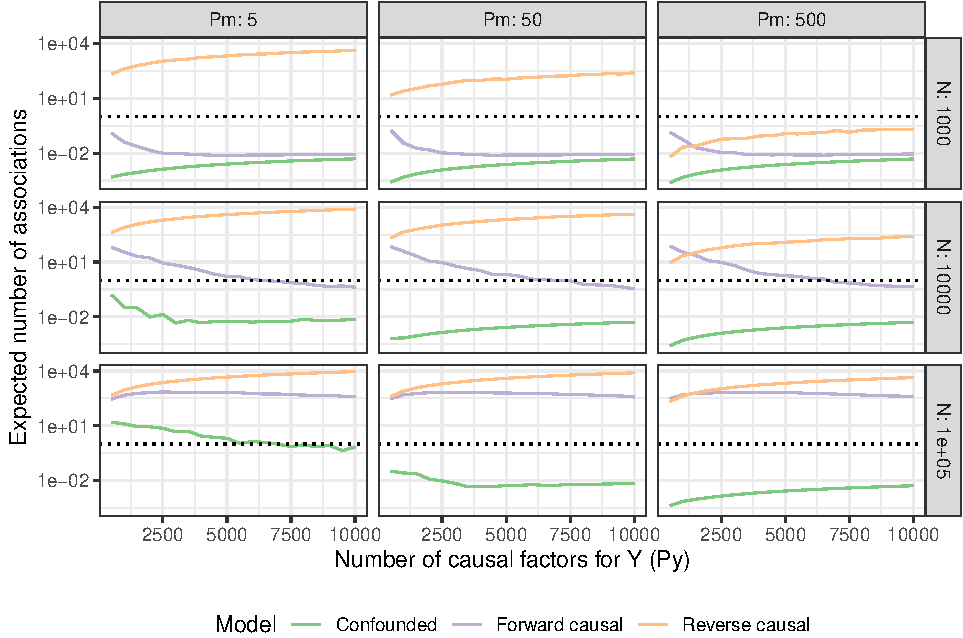
\includegraphics{supplementary-note-EWAS-power_files/figure-latex/pwr-to-detect-assoc-fig-1.pdf}
\caption{\label{fig:pwr-to-detect-assoc-fig}Each box represents the expected number of EWAS associations (y-axis, note the log scale) against how multi-factorial the trait is (x-axis) for the given parameters under each of the three causal models. Rows of boxes represent different sample sizes, and columns of boxes represent how multi-factorial the DNAm sites are. The black dotted line depicts the location on the y-axis for detecting a single causal variant, drawn for convenience.}
\end{figure}

\hypertarget{summary}{%
\section{Summary}\label{summary}}

In general, the power to detect EWAS associations whereby the complex trait of interest influences DNA methylation at a given site (reverse causal), greatly exceeds the power to detect DNA methylation changes that effect the trait (forward causal) when the trait is substantially more multi-factorial than each of the DNA methylation sites. EWAS typically have the least power to detect associations arising due to confounding, though this assumes that each confounder has a small effect on the trait (\(y\)).

\end{document}
